\chapter{Results}
\label{chapter:results}

This chapter gives answers to the questions from chapter~\ref{chapter:introduction}. To answer the methods described in this work, such as approximation, clustering and outlier detection, are combined and used.

\section{Proposed algorithm for Detecting Activated T Cells}
\label{sec:proposed-algorithm}

The first and most relevant question was ''Which criteria can distinguish between unactivated, activated and pre-activated cells?''.

First we give a method for filtering the pre-activated cells from a dataset. From their nature we expect a high value in \Calcium concentration at the start of the recording. Using the approximation from chapter~\ref{chapter:approximating} it is easy to get the approximate \Calcium concentration value at the start of the recording, as it is the parameter $u$. Using the algorithm~\ref{alg:outlier_detection} with parameters threshold as $[\infty, 0.5]$ and parameters\_used as [$u$] gives good results. It returns the indices of particles, which are pre-activated in the data sets of the positive controls.

After having filtered out pre-activated particles, we want to distinguish between unactivated and activated particles. For this we propose the following steps:

\begin{enumerate}
	\item get positive control, negative control and experiment recordings
	\item transform each particle time series of all three data sets to the parameter list by approximating it with a combination of sigmoid functions, according to chapter~\ref{chapter:approximating}, using the algorithm \ref{alg:main}
	\item normalize each of the parameters of all data sets
	\item use outlier detection, which is described in algorithm~\ref{alg:outlier_detection}, to filter out non-conforming cells from both the positive and negative control, as well as pre-activated cells, and particles where the approximation yielded suboptimal results
	\item sample particles from the filtered positive and negative control groups to match the number of particles in the both groups
	\item use clustering method, as one described in chapter~\ref{chapter:clustering}, with parameters of selected negative and positive control as input to get the clustering parameters
	\item predict the membership of the experiment particle parameters to the clusters to get a prediction of activation
\end{enumerate}

The third and fifth step is beneficial when clustering, as many clustering methods expect equally sized clusters that are centred and have equal standard deviation. 

This algorithm is implemented in Python and shown in appendix~\ref{chapter:python_implementation}. Applying this to three data sets of mouse t cells gives the exemplary results shown in table~\ref{tab:results_main_algorithm}. The number of activated cells detected in the positive and negative control are shown as a reference point. Comparing them in the case illustrated suggests that in this case Gaussian Mixture Model is the better clustering algorithm.

\begin{table}[h]
	\centering
	\begin{tabular}{|c|c|c|c|c|}
		\hline
		 & file & activated & out of & percentage\\
		 \hline
		  & negative control & 47 & 969 & 4.850\\
		 gaussian mixture & positive control & 932 & 969 & 96.182\\
		  & experiment & 716 & 890 & 80.449\\
		 \hline
		  & negative control & 53 & 969 & 5.470\\
		 kmeans & positive control & 926 & 969 & 95.562\\
		  & experiment & 687 & 890 & 77.191\\
		 \hline
	\end{tabular}
	\caption{Output of the proposed algorithm applied to three files of mouse t cells.}
	\label{tab:results_main_algorithm}
\end{table}

The algorithm can be adapted by using different clustering methods, or specifying other methods of separating the particles based on the parameters derived.

\section{Difference between Mouse and Human Cells}
\label{sec:differences_between_mouse_and_human_cells}

Now that we have an algorithm for detecting activated cells, we might ask whether there are notable differences between mouse and human cells. Plotting all data points in a single plot, as seen in figure~\ref{fig:all_cells}, shows whether differences are to be expected.

\begin{figure}[h]
	\centering
	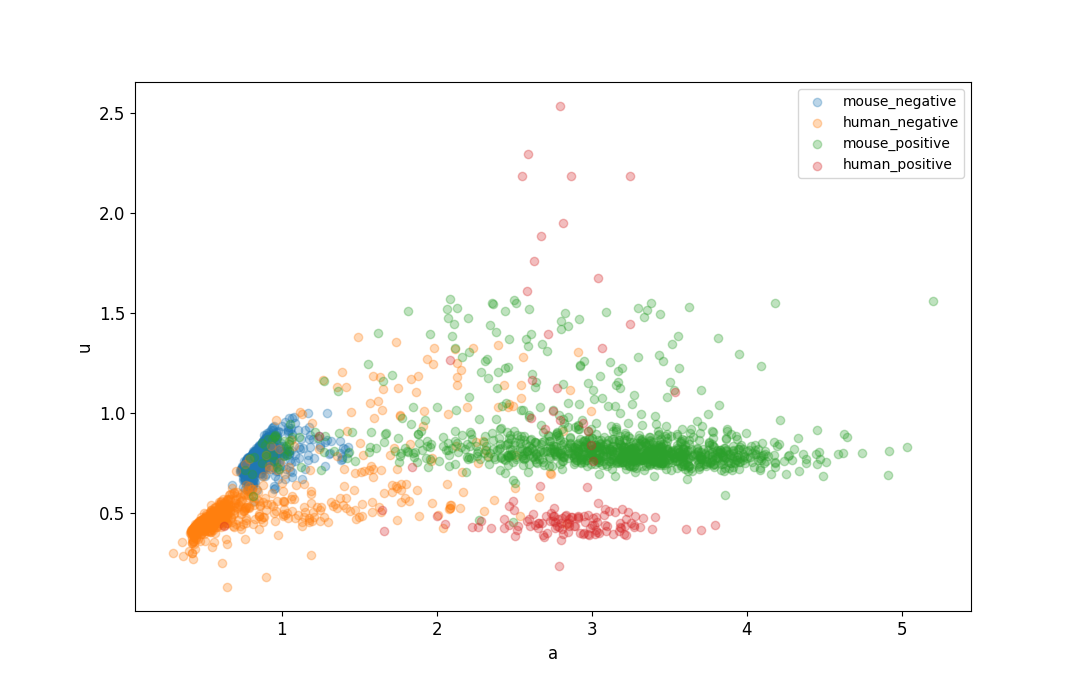
\includegraphics[width=0.8\textwidth]{fig/all_cells}
	
	\caption{All data points from the four control data sets plotted along the axes activated value $a$ and unactivated values $u$.}
	\label{fig:all_cells}
\end{figure}

This shows differences in the axes $a$ and $u$ are present. On average the unactivated value $u$ and activated value $a$ are bigger in mouse t cells than the human counterparts.

[TODO explain table below]

\begin{table}[h]
	\centering
	\begin{tabular}{|c|c|c|c|c|c|c|c|c|c|}
		\hline
		& & & a & u & d & k1 & k2 & w1 & w2\\
		\hline
		\multirow{4}{*}{\rotatebox[origin=c]{90}{mouse}} & \multirow{2}{*}{\rotatebox[origin=c]{90}{pos}} & $\mu$ & 0.94 & 0.333 & 0.92 & -0.569 & 0.12 & 0.778 & 0.535\\
		\cline{3-10}
		& & $\sigma$ & 0.298 & 1.614 & 0.37 & 0.004 & 0.303 & 0.315 & 0.336\\
		\cline{2-10}
		& \multirow{2}{*}{\rotatebox[origin=c]{90}{neg}} & $\mu$ & -0.904 & -0.32 & -0.884 & 0.546 & -0.115 & -0.747 & -0.514\\
		\cline{3-10}
		& & $\sigma$ & 0.007 & 0.201 & 0.012 & 1.348 & 1.642 & 0.519 & 1.098\\
		\hline
		\multirow{4}{*}{\rotatebox[origin=c]{90}{human}} & \multirow{2}{*}{\rotatebox[origin=c]{90}{pos}} & $\mu$ & 0.826 & 0.173 &  0.75 & -0.271 & 0.259 & -0.201 &	-0.252\\
		\cline{3-10}
		& & $\sigma$ & 0.167 & 1.54 & 0.456 & 0.073 & 0.097 & 0.311 & 0.677\\
		\cline{2-10}
		& \multirow{2}{*}{\rotatebox[origin=c]{90}{neg}} & $\mu$ & -1.069 & -0.224 & -0.97 & 0.351 & -0.336 & 0.26 &	0.327 \\
		\cline{3-10}
		& & $\sigma$ & 0.052 & 0.212 & 0.036 & 1.982 & 1.969 & 1.772 & 1.229\\
		\hline
	\end{tabular}
	\caption{Means and standard deviations of the positive and negative controls in human and mouse cells output from using Gaussian Mixture Model. The values in the rows marked with $\sigma$ are the values in the diagonal of the covariance matrix.}
	\label{tab:mean_std_clustering}
\end{table}

[TODO Compare mean and covariance between the mouse and human.]

[TODO same with kmeans instad of gaussian mixture model]


\section{Oscillation in Decrease}

Question: With which frequencies does the Calcium concentration repeat after activation?

Answer: Results from frequency analysis

\section{Types of Activated Cells}

We are interested in whether there are different types of activated cells. The question formulated in chapter~\ref{chapter:introduction} is ''Do different types of activated cells exists? How are they different?''

We find an answer by looking at the activated cells only. We have two data sets of activated cells, one from mouse cells and one from human cells. Naturally there will be differences between the two. This was further explored in section~\ref{sec:differences_between_mouse_and_human_cells}. By looking at only one data set of the positive control at a time we generate the images seen in figure~\ref{fig:positive_control}. To reduce the dimensionality once again Principal Component Analysis is used.

\begin{figure}[h]
	\centering
	\begin{subfigure}{0.49\linewidth}
		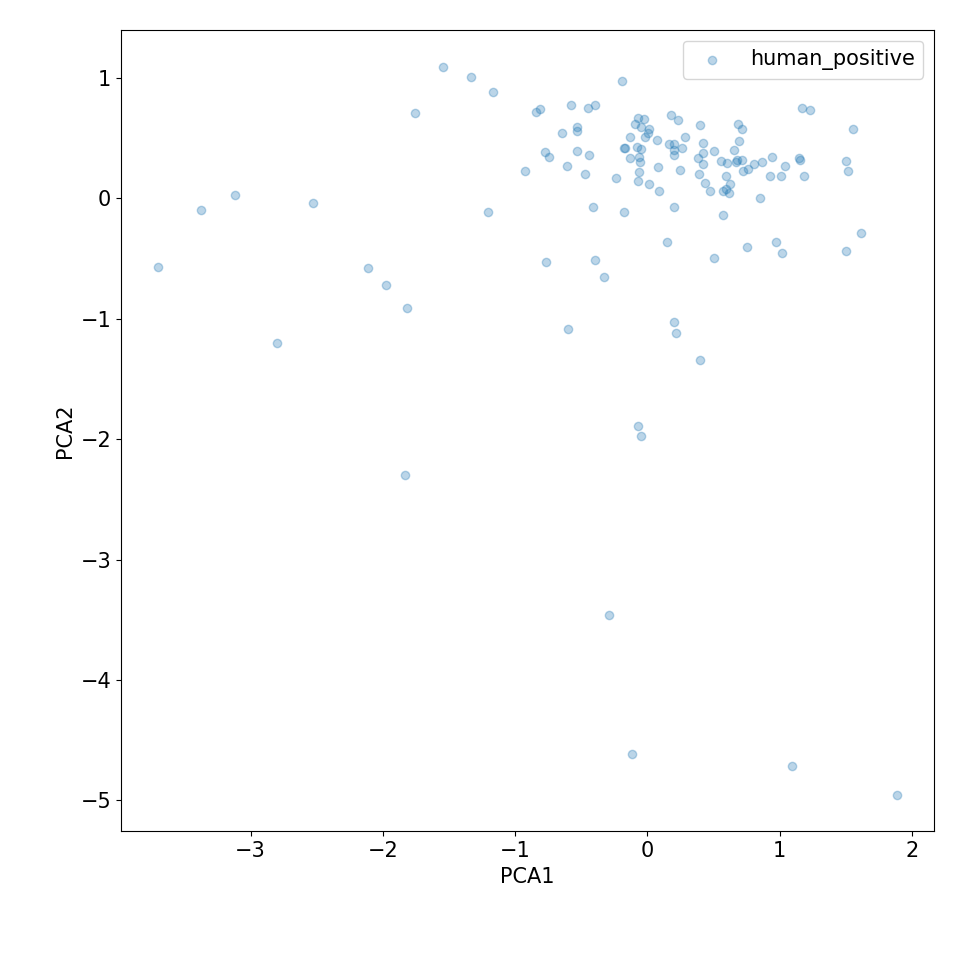
\includegraphics[width=\textwidth]{fig/positive_control_human}
	\end{subfigure}
	\hfill
	\begin{subfigure}{0.49\linewidth}
		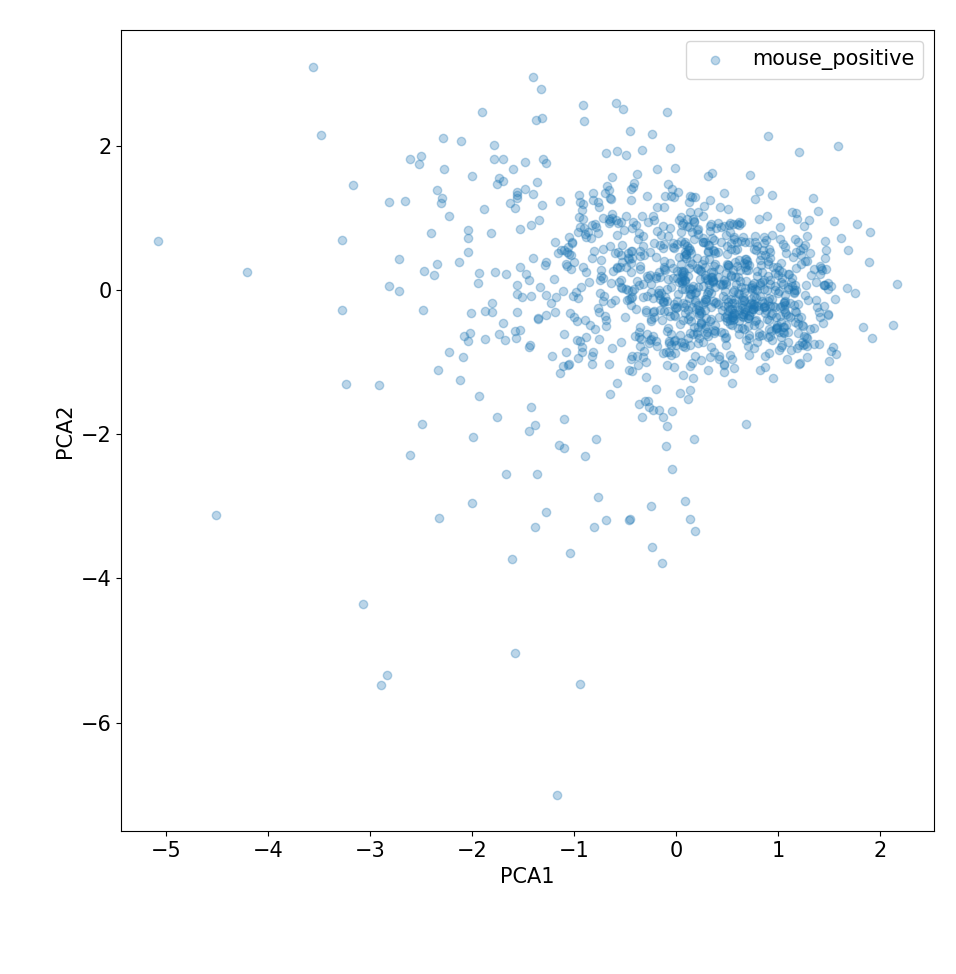
\includegraphics[width=\textwidth]{fig/positive_control_mouse}
	\end{subfigure}
	
	\caption{First two axes of the Principal Component Analysis of activated human and mouse t cells.}
	\label{fig:positive_control}
\end{figure}

From figure~\ref{fig:positive_control}, it is not apparent that there are different types of activated cells.

[TODO see if using oscillations shows differences]